%-----------------------------------------------------------------------------%
\chapter{\babEmpat}
%-----------------------------------------------------------------------------%
Bagian ini berisi penjelasan mengenai implementasi program-program yang terkait dengan penelitian. Program tersebut meliputi perkalian matriks, kovolusi matriks, transpose matriks, serta penjumlahan matriks yang diimplementasikan menggunakan OpenCL dan diintegrasikan ke Tensorflow Lite. 

%-----------------------------------------------------------------------------%
\section{OpenCL Matriks Multiplication}
%-----------------------------------------------------------------------------%
Ukuran blok yang digunakan disesuaikan dengan ukuran work-group yang disarankan pada OpenCL. Pada umunya perangkat android menyarankan ukuran kelipatan 8, sehingga ukuran blok dapat diambil 8x8, 16x32 atau 32x32. Ukuran lebih besar dari 32 tidak disarankan karena mayoritas perangkat memiliki batas jumlah work-item dalam suatu work-group sebanyak 1024 (32x32).
///////////

Implementasi perkalian matriks menggunakan blocking matrix multiplication. Kedua matriks yang dikalikan dibagi ke dalam beberapa block yang sama dimana satu block memiliki ukuran 32x32. Perhatikan pada gambar , terdapat dua matriks A dan B yang masing-masing berukuran MxK dan KxN. Dengan demikian perkalian keduanya menghasilkan matriks C yang berukuran MxN. Blok pada matriks C yang berwarna ungu diperoleh dari dua tahap perkalian matriks, yaitu perkalian antara blok hijau muda dan blok biru muda pada matriks A dan B kemudian ditambahkan dengan perkalian antara blok hijau tua dan blok biru tua pada matriks A dan B.

\begin{figure}
	\centering
	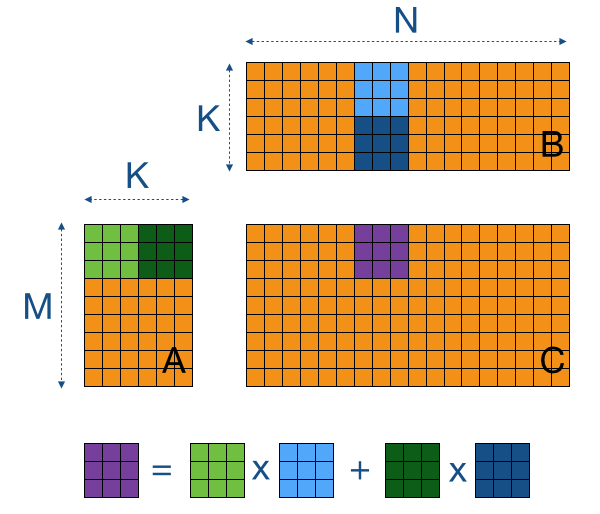
\includegraphics[width=0.50\textwidth]
	{pics/matmul-block1.png}
	\caption{Perkalian matriks per blok.}
	\label{fig:matmulblock}
\end{figure}

Motivasi dari penggunaan blok pada perkalian matriks adalah untuk meningkatkan efisiensi penggunaan cache pada GPU. Perhatikan bahwa untuk mendapatkan suatu elemen baris ke i dan kolom ke j dari matriks, baris ke i dari matriks A dan kolom ke j dari akan diload ke memory dan cache. Kemudian untuk mendapatkan suatu elemen baris ke i+1 dan kolom ke j dari matriks, kolom ke j dari matriks B kembali diload ke memory. Kolom ke j dari matriks B ini selalu digunakan ulang dalam menghitung elemen kolom ke j pada matriks C.

Untuk matriks berukuran besar, besar kemungkinan bahwa kolom tersebut sudah terhapus dari cache karena sebelum memproses kolom itu lagi, cache terlebih dahulu digunakan untuk menyimpan kolom-kolom lain karena sudah banyak perkalian yang dilakukan. Sedangkan ketika matriks berukuran kecil, peluang kolom tersebut masih berada di cache lebih tinggi, sehingga komputasi menggunakan kolom tersebut menjadi lebih cepat. Inilah mengapa matriks dibagi ke dalam beberapa bagian yang lebih kecil untuk dikalikan secara bertahap agar frekuensi penggunaan cache lebih tinggi sehingga komputasi lebih cepat. 

Perkalian per blok ini dapat diimplementasikan dalam OpenCL kernel seperti berikut. Iterasi dilakukan sebanyak K/blocksize kali. Pada setiap iterasi, perkalian per blok dilakukan untuk 32 kolom dari matriks A (semua baris) dan 32 baris dari matriks B (semua kolom). Ingat bahwa ukuran blok adalah 32x32.

\begin{lstlisting}[frame=single]
__kernel void matrixVectorMul(__global float* C, 
    const __global float* A, 
    const __global float* B, 
    int K, int M, int N) { 

	// Local row ID (max: 32)
    const int row = get_local_id(0);
    // Local col ID (max: 32)  
    const int col = get_local_id(1);
    // Row ID of C (0..M)  
    const int globalRow = 32*get_group_id(0) + row; 
    // Col ID of C (0..N) 
    const int globalCol = 32*get_group_id(1) + col;  

    __local float Asub[32][32]; 
    __local float Bsub[32][32]; 

    float acc = 0.0; 

    const int numTiles = ((K-1)/32)+1; 
    for (int t=0; t<numTiles; t++) { 

        const int tiledRow = 32*t + row; 
        const int tiledCol = 32*t + col; 
        if((tiledCol < K) && (globalRow < M)) {
            Asub[col][row] = A[globalRow*K + tiledCol]; 
        }  
        else {   
            Asub[col][row] = 0.0; 
        }  
        if((tiledRow < K) && (globalCol < N)) {
            Bsub[col][row] = B[globalCol*K + tiledRow]; 
        }  
        else {   
            Bsub[col][row] = 0.0; 
        }  

        barrier(CLK_LOCAL_MEM_FENCE); 

        for (int k=0; k<32; k++) { 
            acc += Asub[k][row] * Bsub[col][k]; 
        } 

        barrier(CLK_LOCAL_MEM_FENCE); 
    } 

    if((globalRow < M) && (globalCol < N)) { 
        C[globalCol*M + globalRow] = acc; 
    }
}
\end{lstlisting}

%-----------------------------------------------------------------------------%
\section{OpenCL Matriks Convolution}
%-----------------------------------------------------------------------------%

%-----------------------------------------------------------------------------%
\section{Vulkan Matriks Multiplication}
%-----------------------------------------------------------------------------%
Implementasi perkalian matriks menggunakan blocking matrix multiplication. Kedua matriks yang dikalikan dibagi ke dalam beberapa block yang sama dimana satu block memiliki ukuran 32x32. Perhatikan pada gambar , terdapat dua matriks A dan B yang masing-masing berukuran MxK dan KxN. Dengan demikian perkalian keduanya menghasilkan matriks C yang berukuran MxN. Blok pada matriks C yang berwarna ungu diperoleh dari dua tahap perkalian matriks, yaitu perkalian antara blok hijau muda dan blok biru muda pada matriks A dan B kemudian ditambahkan dengan perkalian antara blok hijau tua dan blok biru tua pada matriks A dan B.

\begin{figure}
	\centering
	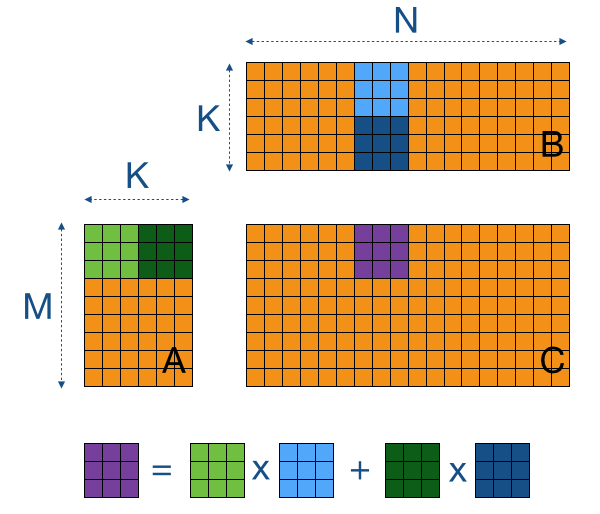
\includegraphics[width=0.50\textwidth]
	{pics/matmul-block1.png}
	\caption{Perkalian matriks per blok.}
	\label{fig:matmulblock}
\end{figure}

Motivasi dari penggunaan blok pada perkalian matriks adalah untuk meningkatkan efisiensi penggunaan cache pada GPU. Perhatikan bahwa untuk mendapatkan suatu elemen baris ke i dan kolom ke j dari matriks, baris ke i dari matriks A dan kolom ke j dari akan diload ke memory dan cache. Kemudian untuk mendapatkan suatu elemen baris ke i+1 dan kolom ke j dari matriks, kolom ke j dari matriks B kembali diload ke memory. Kolom ke j dari matriks B ini selalu digunakan ulang dalam menghitung elemen kolom ke j pada matriks C.

Untuk matriks berukuran besar, besar kemungkinan bahwa kolom tersebut sudah terhapus dari cache karena sebelum memproses kolom itu lagi, cache terlebih dahulu digunakan untuk menyimpan kolom-kolom lain karena sudah banyak perkalian yang dilakukan. Sedangkan ketika matriks berukuran kecil, peluang kolom tersebut masih berada di cache lebih tinggi, sehingga komputasi menggunakan kolom tersebut menjadi lebih cepat. Inilah mengapa matriks dibagi ke dalam beberapa bagian yang lebih kecil untuk dikalikan secara bertahap agar frekuensi penggunaan cache lebih tinggi sehingga komputasi lebih cepat. 

Perkalian per blok ini dapat diimplementasikan dalam OpenCL kernel seperti berikut. Iterasi dilakukan sebanyak K/blocksize kali. Pada setiap iterasi, perkalian per blok dilakukan untuk 32 kolom dari matriks A (semua baris) dan 32 baris dari matriks B (semua kolom). Ingat bahwa ukuran blok adalah 32x32.

\begin{lstlisting}[frame=single]
__kernel void matrixVectorMul(__global float* C, 
const __global float* A, 
const __global float* B, 
int K, int M, int N) { 

// Local row ID (max: 32)
const int row = get_local_id(0);
// Local col ID (max: 32)  
const int col = get_local_id(1);
// Row ID of C (0..M)  
const int globalRow = 32*get_group_id(0) + row; 
// Col ID of C (0..N) 
const int globalCol = 32*get_group_id(1) + col;  

__local float Asub[32][32]; 
__local float Bsub[32][32]; 

float acc = 0.0; 

const int numTiles = ((K-1)/32)+1; 
for (int t=0; t<numTiles; t++) { 

const int tiledRow = 32*t + row; 
const int tiledCol = 32*t + col; 
if((tiledCol < K) && (globalRow < M)) {
Asub[col][row] = A[globalRow*K + tiledCol]; 
}  
else {   
Asub[col][row] = 0.0; 
}  
if((tiledRow < K) && (globalCol < N)) {
Bsub[col][row] = B[globalCol*K + tiledRow]; 
}  
else {   
Bsub[col][row] = 0.0; 
}  

barrier(CLK_LOCAL_MEM_FENCE); 

for (int k=0; k<32; k++) { 
acc += Asub[k][row] * Bsub[col][k]; 
} 

barrier(CLK_LOCAL_MEM_FENCE); 
} 

if((globalRow < M) && (globalCol < N)) { 
C[globalCol*M + globalRow] = acc; 
}
}
\end{lstlisting}

%-----------------------------------------------------------------------------%
\section{Vulkan Matriks Convolution}
%-----------------------------------------------------------------------------%